\chapter{An introduction to OSGi}


\section{Java's limitations of modularity}
Java platform, which was first introduced in 1995, has become highly popular. It is used to develop many kinds of applications, from mobile to desktop, enterprise. Java programming is highly object-oriented, it contains a number of good features, which are encapsulation, abstraction, inheritance, polymorphism. Those features make applications more dynamic and modular, compared to others used older technologies than Java. However, when applications become massive in size, more complex in logic, such features are not sufficient to scale these applications. The reason is that Java platform itself does not fully support modularity.

\subsection{Java's encapsulation}
With the principle of encapsulation, at class-level, Java have a mechanism to control visibility of classes and class members, which are properties and methods or classes themselves, by using access modifiers including public, protected, private or none indicating package level. This appears that we are able to create more independent classes, then the application tends to be more modular since it is made of many classes?

However, this level of encapsulation is only for low-level, individual classes. As classes are logically grouped together into packages that are typically used in Java organize code which is related in some way, this kind of encapsulation does not work well to make the whole application more modular. For code to be used from one package to another, the code must be declared public or protected using inheritance. 

Normally, a package uses code from different others, which means the implementation in outside packages must be exposed as public. So it turns out that when two packages communicate with another one, they have to know public APIs (Java interfaces) and private implementation as well. Which proves that packages are more dependent on each other the whole system is hard to change or less modular. The problem here is how two modules collaborate just by knowing a public APIs.

\subsection{Java class-path}
As mentioned above, Java code is usually placed into packages, then after being compiled, packages are also packed into JAR files which are a way to use code as libraries or parts of an application. 

Since an application is composed by JAR files, when classes are about to be used, it must be located in a bundle of JAR files by the compiler to set up Java class path, which tells where the needed classes are. Unfortunately, a JAR file does not give any information about the code inside it, such as versions, dependencies. The process of finding classes in JARs to set up class path is completely trial and error, and it continues until the required classes are found. In fact, Java class path returns the first version of the code it finds. 

To give an example, a Java class in an application requires a set of classes organized in a package called A, while package A is packed in JAR file 1 and JAR file 2 with two different versions and both files are declared in the application's class path, maybe use class-path variable or MANIFEST file. The question is which version of package A will be used, from JAR 1 or JAR 2, the fact is that if JAR 1 appears first in the class path, then undoubtedly package A in JAR 1 is going to be used. It proves that other versions of package A are overlapped by the one that first appears. Apparently, Java class path pays no attention to the logical version of the code or JAR files. This possibly leads to  errors, like NoSuchMethodError exception, when a class from a JAR file interacts with an incompatible version of code from another. As a result, the consistency of source code is not ensured. Therefore, although a Java application is formed of JAR files, it does not has a highly modular architecture.


\subsection{What is modularity?}
So what is modularity? And why it is so important to large applications?

The term modularity can be explained that a big system is broken in to a number of parts called modules. Each module contains a separate logical content or has a logical boundary, which means that a piece of code is inside only one module and not others. In addition, the details of implementation in a module are visible only to code that is part of the same module. Modules in a system coordinate and communicate in standard ways to make the whole system work. 

\begin{figure}
	\centering
		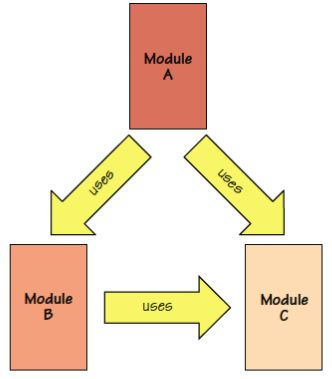
\includegraphics{image/modules.JPG}
	\caption{A large system divided into collaborating modules}
	\label{fig:modules}
\end{figure}

Since modules all have a boundary, they are less dependent on each other, then replacing a module is easy and causes little effect on other parts. Therefore, the system is easy to change or expand, just by replacing or adding modules. Developing software modularily means writing complete modules and assembling them together, which would simplify development and improve maintainability.

\section{The OSGi framework}

\subsection{What is OSGi ?}
OSGi is dynamic modular system for Java used to solve the problem of lacking modularity of Java applications. OSGi was first formed in 1999 but for a different purpose, now it is for building dynamic modular Java applications.

OSGi plays a central role for OSGi-based applications, it provides a run-time environment in which modules can be plugged in and interact with others. In fact, OSGi is a specification which defines and describes how OSGi-based applications work, the way OSGi modules interact; thus there are many implementations for the OSGi core framework, such as Apache Felix, Eclipse Equinox, so we can simply choose one to use.

At the present time, there are several non-trivial applications developed with OSGi platform, for example Eclipse IDE, one of the most popular Integrated Development Environments mainly for Java programming language and many others, or Glassfish Application Server v3, the one uses Apache Felix as its run-time. 

\subsection{Benefits of OSGi}
So why is OSGi able to solve the problems that pure Java cannot?

OSGi reduces the complexity of applications by dividing them into many modules, but this is not the key factor that leads the applications to be more modular. OSGi goes further than that, it has some techniques to make modules less dependent on others, more encapsulated.

Fist of all, each OSGi module has a explicit logical version or code in a module is always assigned a clear version, which is convenient for managing and using code later.

Secondly, a module can explicitly exposes any part of code or none to the public, which means other modules only have the access to the part that is published. Typically, Java interfaces will be seen from the outside, but the implementation will not and two different modules still work well together, whereas we cannot achieve this with pure Java.

Thirdly, an OSGi module also have the control of which version of code it intends to use, which means that a module will refuse to interact with another unless the right version of the code it required is provided. This mechanism avoids the possibility of being inconsistent when incompatible code versions are given to a module.

Along with the above things, OSGi modules communicate in a standard way using exposed interfaces. With each public interface, a service is provided, which is simply a Java object and can be only used through the interface that the object is registered under. Therefore, modules in OSGi have loose relationships, fewer dependencies. This helps the whole system to be more dynamic, more modular, then easy to change, expand as well as develop.

Moreover, another remarkable advantage of OSGi is that removing, adding or replacing modules can be done on the fly or dynamically. There is no need stop a running system to perform the above operations. 
